\documentclass[12pt]{article}
\usepackage[paper=letterpaper,margin=2cm]{geometry}

\usepackage{mathtools, amssymb, amsthm}
\usepackage{enumerate}
\usepackage{enumitem}
\usepackage{fancyhdr}
\usepackage{tabularx}

\pagestyle{fancy}
\fancyhf{}
\rhead{\small {© 2022 All Rights Reserved, Aiden Rosenberg}}
\rfoot{Page \thepage}

%\setlength{\droptitle}{-6em}
\everymath{\displaystyle}

\title{Final Exam Practice}
\author{Aiden Rosenberg}
\date{November 28, 2022 A.D}
\newcommand{\dydx}{\frac{dy}{dx}}

\begin{document}
\maketitle
\begin{enumerate}
    \item If $f(x)=\cos^2(3x-5)$, then $f'(x)=$
    $$f'(x)=2\cos(3x-5)\cdot -\sin (3x-5) \cdot 3 = \boxed{-6\cos(3x-5)\sin(3x-5)}$$
    \item $\int\frac{dt}{t\sqrt{t}} = $
    $$\int \frac{dt}{t^{3/2}} = \int t^{-3/2}\,dt = \boxed{-2t^{-1/2}+C}$$
    \item If $f(x)=\frac{5-x}{x^3+2}$ then $f'(x)=$
    $$f'(x)=\frac{-(x^3+2)-(3x^2)(5-x)}{(x^3+1)^2}=\boxed{\frac{2x^3-15x^2-2}{(x^3+1)^2}}$$
    \item 
    \begin{center}
        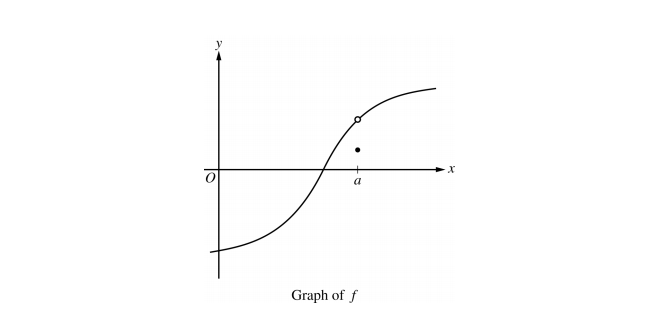
\includegraphics[width=6in]{FEP1.png}
    \end{center}
    The graph of $y = f(x)$ is shown above. Which of the following is true?
    \item If $\int_{4}^{-10} g(x) \, dx = -3$ and $\int_{4}^{6} g(x) \, dx = 5$, then $\int_{-10}^{6} g(x)\, dx = $
    $$\int_{-10}^{6} g(x) \, dx = \int_{-10}^{4} g(x)\, dx + \int_{4}^{6} g(x)\, dx = 3 + 5 = \boxed{8}$$
    \item The slope of the line tangent to the graph of $y=xe^x$ at $x = \ln 2$ is
    $$y'= e^x+xe^x \biggr\rvert_{\ln 2} = \boxed{2+2\ln 2}$$
    \item Let $y = f(x)$ be the solution to the differential equation $\frac{dy}{dx}=x-y$ with initial condition $f(2) = 8$. What is the approximation for $f(3)$ obtained by using Euler's method with two steps of equal length, starting at $x = 2$?
    \begin{table}[h]
        \centering
        \caption{$\Delta x = 0.5$}
        \begin{tabular}{l|l|l|l}
        $x$ & \multicolumn{1}{l|}{$y$} & \multicolumn{1}{l|}{$\frac{dy}{dx}$} & $\Delta y$ \\ \hline
        2 & 8 & -6 & -3 \\
        2.5 & 5 & -2.5 & -1.25 \\
        3 & 3.75 &  & 
        \end{tabular}
        \end{table}
        $$f(3)\approx 3.75 = \boxed{\frac{15}{4}}$$
    \item If $x^2+xy-3y=4$, then at the point $(2, 1)$, $\frac{dy}{dx}=$
    $$2x+y+x\frac{dy}{dx}-3\frac{dy}{dx}=0 \Longrightarrow \frac{dy}{dx} = \frac{-2x-y}{x-3}\bigg\rvert_{(2,1)} = \boxed{5}$$
    \item $\int \frac{3x+1}{x^2-4x+3} \, dx=$
    $$\int \frac{3x+1}{x^2-4x+3} \, dx= \int \frac{3x+1}{(x-1)(x-3)} \, dx = \int \Biggr(\frac{-2}{(x-1)} + \frac{5}{x-3} \Biggr) \, dx$$ 
    $$= \boxed{ -2\ln|x-1|+5\ln|x-3|+C}$$
    \item Which of the following is a slope field for the differential equation $\frac{dy}{dx}=x^2+y^2$?
        \begin{center}
            \boxed{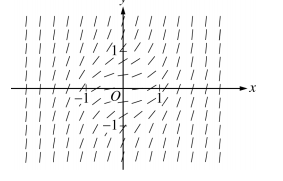
\includegraphics[width=3in]{FEPA1.png}}
        \end{center}
    \item If $f(x) = 3x^2 + 2x$, then $f'(x) =$
    $$\boxed{\lim_{h\to 0} \frac{\big(3(x+h)^2+2(x+h)\big)-(3x^2+2x)}{h}}$$
    \item 
        \begin{center}
            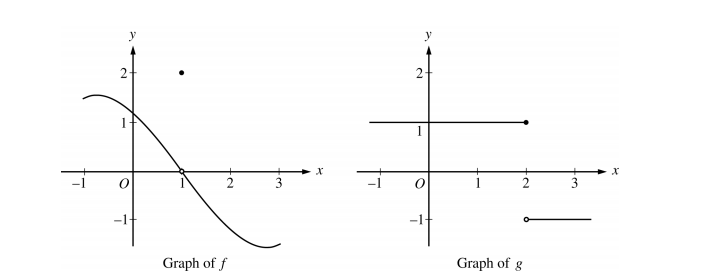
\includegraphics[width=4in]{FEP2.png}
        \end{center}
    The graphs of the functions $f$ and $g$ are shown in the figures above. Which of the following statements is false?
    $$\boxed{\lim_{x \to 1} \big(f(x)\cdot g(x+1) \big) \text { does not exist}}$$
    \item $\int_0^5 \sqrt{\frac{5-x}{5}} \, dx = $
    \begin{enumerate}
        \item Let $u=\frac{5-x}{5} = 1-\frac{x}{5} \Longrightarrow -5du = dx$
    \end{enumerate}
    $$ \int_0^5 \sqrt{\frac{5-x}{5}} \, dx = 5\int_{0}^{1} \sqrt{u} \, du = 5 \cdot \frac{2x^{3/2}}{3} \bigg\rvert_{0}^{1} =\boxed{\frac{10}{3}}$$
    \item Which of the following limits are equal to $-1$?
        \begin{enumerate}[label=\Roman*.]
            \item $\lim_{x\to0^-} \frac{|x|}{x} = -1$
            \item $\lim_{x\to3} \frac{x^2-7x+12}{3-x} = \lim_{x\to3} - (x-4)=1 $
            \item $\lim_{x\to\infty} \frac{1-x}{1+x} \xRightarrow[]{\text{EBM}} -1$
        \end{enumerate}
        $$\boxed{\text{I and III only}}$$
    \item Let $f$ be the function given by $f(x) = 2\cos x + 1$. What is the approximation for $f(1.5)$ found by using the line tangent to the graph of $f at x=\frac{\pi}{2}$?
    $$f\big(\frac{\pi}{2}\big) =2\cos\big(\frac{\pi}{2}\big) +1 = 1$$
    $$f'(x)= -2\sin x$$
    $$f'(\frac{\pi}{2}\big)= -2$$
    $$y = -2\big(x-\frac{\pi}{2})+1 \bigg\rvert_{x=\frac{3}{2}} = \boxed{\pi -2}$$
    \item  
        \begin{table}[h!]
            \centering
            \begin{tabular}{|l||l|l|l|l|}
            \hline
                Time (weeks) & 0   & 2   & 6   & 10  \\ \hline
                Level        & 210 & 200 & 190 & 180 \\ \hline
                \end{tabular}
                \end{table}
    The table above gives the level of a person's cholesterol at different times during a 10-week treatment period. What is the average level over this 10-week period obtained by using a trapezoidal approximation with the subintervals $[0, 2]$, $[2, 6]$, and $[6, 10]$?
    $$f_{avg}= \frac{(210+200)+2(200+190)+2(180+190)}{10} = \boxed{193}$$
    \item $\int \frac{xe^{\frac{-3x}{4}}}{2}, dx$
    \begin{enumerate}
        \item Let $u=\frac{x}{2} \Longrightarrow du = \frac{1}{2} dx$
        \item Let $dv = e^{\frac{-3x}{4}} \Longrightarrow v= \frac{-4}{3}e^{\frac{-3x}{4}}$
    \end{enumerate}
    $$\Longrightarrow \frac{-2x}{3}e^{\frac{-3x}{4}} - \int \frac{-4}{6}e^{\frac{-3x}{4}} \, dx = \boxed{\frac{-2x}{3}e^{\frac{-3x}{4}} + \frac{8}{9}e^{\frac{-3}{4}}+C}$$

    \item If the average value of a continuous function $f$ on the interval $[-2, 4 ]$ is $12$, what is $\int_{-2}^{4} \frac{f(x)}{8} \, dx$
    $$12 = \frac{1}{6} \int_{-2}^{4} f(x) \, dx \Longrightarrow 72 = \int_{-2}^{4} f(x) \, dx$$
    $$\int_{-2}^{4} \frac{f(x)}{8} \, dx = \frac{72}{8} =\boxed{9}$$
    \item Let $f$ be the function with $f(0)=\frac{1}{\pi^2}$, $f(2)=\frac{1}{\pi^2}$, and derivative given by $f'(x)=(x+1)\cos(\pi x)$. How many values of $x$ in the open interval $(0, 2)$ satisfy the conclusion of the Mean Value Theorem for the function $f$ on the closed interval $[0, 2]$?
    $$\cos(\pi x) = \text{ when } x = \frac{1}{2} \text{ and } x= \frac{3}{2}$$
    $$\boxed{\text{Two}}$$
    \item The number of students in a cafeteria is modeled by the function $P$ that satisfies the logistic differential equation $\frac{dP}{dt}=\frac{1}{2000}P(200-P)$, where $t$ is the time in seconds and $P(0) = 25$. What is the greatest rate of change, in students per second, of the number of students in the cafeteria?
    $$\frac{dP}{dt}= \frac{P}{10}-\frac{P^2}{2000}$$
    $$\frac{d^2P}{dt^2} = \frac{1}{10}-\frac{P}{1000}$$
    $$\frac{d^2P}{dt^2} = 0 \text{ when } P=100$$
    $$\frac{dP}{dt}\bigg\rvert_{P=100} = \boxed{5}$$
    \item A cube with edges of length $x$ centimeters has volume $V(x) = x^3$ cubic centimeters. The volume is increasing at a constant rate of $40$ cubic centimeters per minute. At the instant when $x = 2$, what is the rate of change of $x$, in centimeters per minute, with respect to time?
    $$\frac{dV}{dt}= 3x^2 \cdot \frac{dx}{dt} \Longrightarrow \frac{dx}{dt} = \frac{dV}{dt} \cdot \frac{1}{3x^2}\biggr\rvert_{x=2}= \frac{40}{12} = \boxed{\frac{10}{3}}$$
    \item Let $f$ be a twice-differentiable function for all real numbers $x$. Which of the following additional properties guarantees that $f$ has a relative minimum at $x = c$?
    $$\boxed{f'(c) = 0 \text{ and } f''(c) > 0}$$
    \item Let $H(x)$ be an antiderivative of $\frac{x^3+\sin x}{x^2+2}$. If $H(5) = \pi$, then $H(2) =$
    $$H(2) = H(5)-\int_{2}^{5} \frac{x^3+\sin x}{x^2+2} \, dx \approx \boxed{-5.867}$$
    \item The continuous function $f$ is positive and has domain $x > 0$. If the asymptotes of the graph of $f$ are $x = 0$ and $y = 2$, which of the following statements must be true?
    $$\boxed{\lim_{x\to 0^{+}}f(x)= \infty \text{ and } \lim_{x\to\infty} f(x) = 2}$$
    \item 
    \begin{center}
        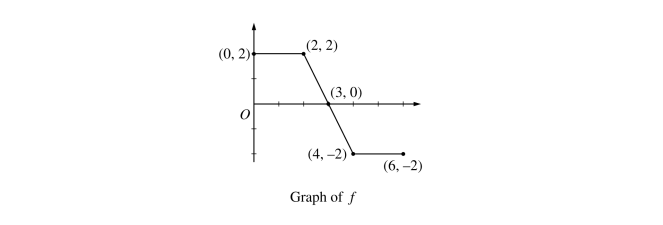
\includegraphics[width=4in]{FEP3.png}
    \end{center}
    The graph of a function $f$, consisting of three line segments, is shown above. The function $f$ is defined on the closed interval $[0, 6]$. Let $g(x) = \int_{2}^{x} f(t) \, dt$. What is the maximum value of $g(x)$ for $0 \leq x \leq 6$?
    $$g'(x)  = \frac{d}{dx}\biggr(\int_{2}^{x} f(t) \, dt\biggr) = f(x)$$
    $$g'(x)=f(x)=0 \text{ when } x= 3$$
    $$\int_{2}^{3} f(t) \, dt = \boxed{1}$$
    \item  
    \begin{center}
        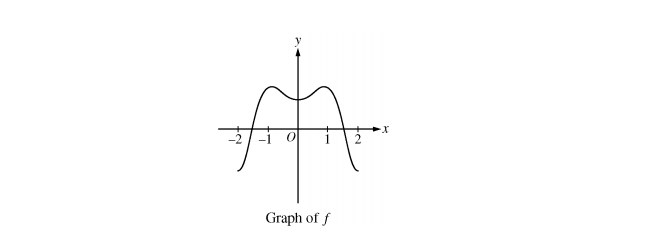
\includegraphics[width=5in]{FEP4.png}
    \end{center}
    The graph of the function $f$ is shown above for $-2 \leq x \leq 2$. Which of the following could be the graph of an antiderivative of $f$?
    \begin{center}
        \boxed{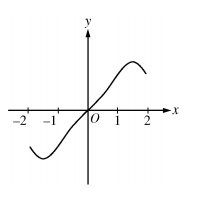
\includegraphics[width=2in]{FEPA2.png}}
    \end{center}
    \item The derivative of the function $f$ is given by $f'(x)=e^{-x}\cos(x^2)$, for all real numbers $x$. What is the minimum value of $f(x)$ for $-1 \leq x \leq 1$?
    $$f'(x) = 0 \text{ when } \cos(x^2) = 0 \Longrightarrow x = \sqrt{\frac{\pi}{2}}$$
    \begin{table}[h]
        \centering
        \begin{tabular}{l|l}
        $x$ & $f(x)$ \\ \hline 
        -1 & $\int_{-1}^{-1} f'(x) \, dx  = 0$ \\ \hline
        $\sqrt{\frac{\pi}{2}}$ &  $\int_{-1}^{\sqrt{\frac{\pi}{2}}} f'(x) \, dx \approx 2.111$ \\ \hline
        1 & $\int_{-1}^{1} f'(x) \, dx\approx 2.087$ \\ 
        \end{tabular}
        \end{table}

$$\boxed{\text{The minimum value of} f(x) \text{ is } f(-1) \text{ justifyed by candidates test.}}$$
    \item 
        \begin{center}
            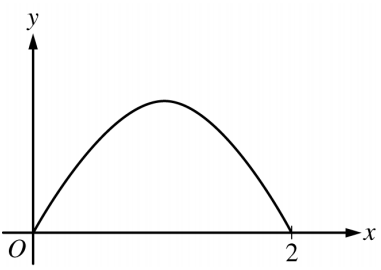
\includegraphics[width=2.5in]{FEP5.png}
        \end{center}
    The base of a solid is the region bounded by a portion of the graph of $y=\sin\bigg(\frac{\pi}{2}x\bigg)$ and the $x$-axis, as shown in the figure above. For the solid, each cross section perpendicular to the $x$-axis is a rectangle of height $3$. Which of the following expressions gives the volume of the solid?
    $$\boxed{3\int_{0}^{2}\sin\bigg(\frac{\pi}{2}x\bigg) \, dx }$$

    \item If $g$ is a twice-differentiable function, where $g(1) = 0.5$ and $\lim_{x\to \infty} g(x) =4$, then $\int_{1}^{\infty} g'(x) \, dx$ is
    $$\int_{1}^{\infty} g'(x) \, dx= \lim_{x\to \infty} g(x)  -g(1)= 4-0.5 = \boxed{3.5} $$

    \item 
        \begin{center}
            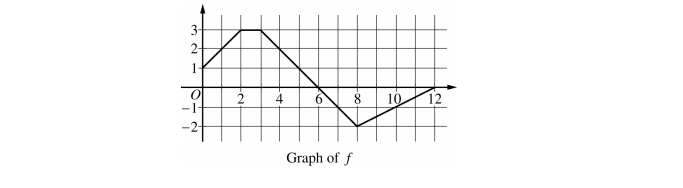
\includegraphics[width=5in]{FEP6.png}
        \end{center}
        The graph of the function $f$ is shown above. If $g$ is the function defined by $g(x)=\int_{2}^{x} f(t) \, dt$, what is the value of $g(10) \cdot g'(10)$?
        \begin{enumerate}
            \item $g(10) = \int_{2}^{10} f(t) \, dt = \frac{5}{2}$
            \item $g'(10)=f(t) = -1$
        \end{enumerate}
        $$g(10) \cdot g'(10) = \boxed{\frac{-5}{2}}$$
    \item 
    \begin{align*}
        f''(x) &= x(x-1)^2(x+2)^3\\
        g''(x) &= x(x-1)^2(x+2)^3 +1\\
        h''(x) &= x(x-1)^2(x+2)^3 -1
    \end{align*}
    The twice-differentiable functions $f$, $g$, and $h$ have second derivatives given above. Which of the functions $f$, $g$, and $h$ have a graph with exactly two points of inflection?
    $$\boxed{f \text{ and } g \text{ only }}$$
    \item The function $f$ is increasing on the interval $[1, 3]$ and nowhere else. The first derivative of $f$, $f'$, is continuous for all real numbers. Which of the following could be a table of values for $f'(x)$?
    \begin{center}
        \boxed{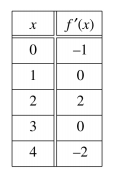
\includegraphics[width=1.5in]{FEPA3.png}}
    \end{center}
    \item If $y=x\sqrt{2x+5}$, then $y'=$
    $$\boxed{y'=\frac{3x+5}{\sqrt{2x+5}}}$$
    \item $\int 2^x \, dx$
    $$\int 2^x \, dx = \frac{2^x}{\ln 2} + C$$
    \item $\lim_{x\to -7} \frac{x+7}{|x+7|}$ is \boxed{\text{nonexistent}}
    \item $\int \frac{(x^{1/3}-4)^5}{6x^{2/3}} \, dx =$
    \begin{enumerate}
        \item Let $u=x^{1/3}-4 \Longrightarrow du = \frac{1}{3x^{2/2}} dx$
    \end{enumerate}
    $$\Longrightarrow \frac{1}{2}\int u^5 \, du = \frac{u^6}{12} +C = \boxed{\frac{(x^{1/3}-4)^6}{12}+C}$$
    \item  
        \begin{table}[h!]
            \centering
            \begin{tabular}{|l||l|l|l|l|}
            \hline
            $t$ (minutes)              & 0   & 5   & 10 & 15 \\ \hline
            $R(t)$ (people per minute) & 100 & 100 & 75 & 55 \\ \hline
            \end{tabular}
        \end{table}
     During an evacuation drill, people leave a building at a rate of $R(t)$ people per minute, where $t$ is the number of minutes since the start of the drill. Selected values of $R(t)$ are shown in the table above. Using a right Riemann sum with three subintervals and data from the table, what is the approximation of the number of people who leave the building during the first 15 minutes of the evacuation drill?
     $$\text{RRAM}_3 = 5\big(100+75+55\big)=\boxed{1500 \text{ people}}$$
     \item If $f(x)=(x^2+1)^3$, what is $\lim_{x\to -1} \frac{f(x)-f(-1)}{x+1}$
     $$f'(1)= \lim_{x\to -1} \frac{f(x)-f(-1)}{x+1} = 6x(x^2+1)^2\bigg\rvert_{x=-1}=\boxed{-24}$$
     \item 
        \begin{center}
            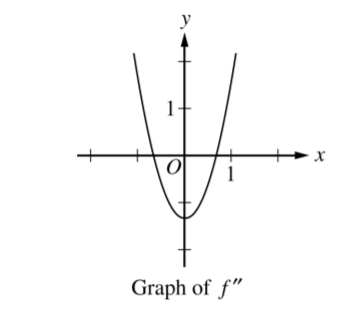
\includegraphics[width=3in]{FEM7.png}
        \end{center}
        The graph of $f''$, the second derivative of the function $f$, is shown above. Which of the following could be the graph of $f$?
        \begin{center}
            \boxed{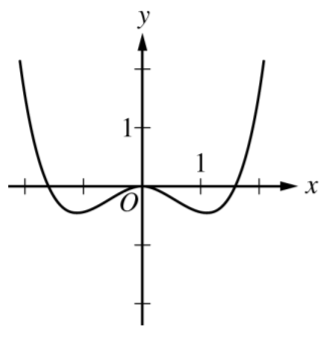
\includegraphics[width=2in]{FEPA4.png}}
        \end{center}
    \item Let $y = f(x)$ be a differentiable function such that   $\frac{dy}{dx}=\frac{x}{y}$   and  $f(8)=2$ . What is the approximation of $f (8.1)$ using the line tangent to the graph of $f$ at $x = 8$?
    $$\frac{dy}{dx}\bigg\rvert_{(8,2)}=4$$
    $$y=4(x-8)+2\bigg\rvert_{x=8.1} = \frac{24}{10}$$
    $$\boxed{f(8.1)\approx 2.4}$$
    \item $\int x\cos(2x) \, dx = $
    \begin{enumerate}
        \item Let $u=x \Longrightarrow du=dx$
        \item Let $$dv= \cos(2x) \longrightarrow v= \frac{\sin (2x)}{2}$$
    \end{enumerate}
    $$\int x\cos(2x) \, dx = \frac{x\sin(2x)}{2}-\int \frac{\sin(2x)}{2}\, dx = \boxed{\frac{x\sin(2x)}{2} + \frac{\cos (2x)}{4}+C}$$
    \item Given that $3x - \tan y = 4$, what is $\frac{dy}{dx}$ in terms of $y$?
    $$3-\sec^2 y \frac{dy}{dx}=0 \Longrightarrow \frac{dy}{dx} = \frac{3}{\sec^2 y}= \boxed{3\cos^2 y}$$
    \item Which of the following graphs is the solution to the logistic differential equation $\frac{dy}{dx}=\frac{y}{5}\bigg(1-\frac{y}{500}\bigg)$ with the initial condition  $y(0) = 100$?
    \begin{center}
        \boxed{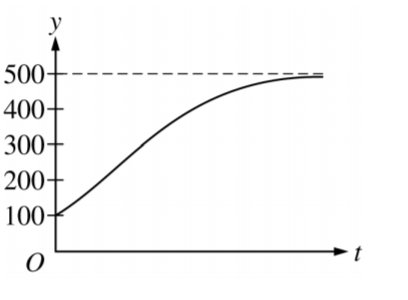
\includegraphics[width=2.5in]{FEPA5.png}}
    \end{center}
    \item What is the absolute minimum value of  $y = -\cos x - \sin x$  on the closed interval $[0,\frac{\pi}{2}]$
    $$y'=\sin x-\cos x$$
    $$y'=0 \Longrightarrow \sin x= \cos x \Longrightarrow x=\frac{\pi}{4}$$
    \begin{table}[h]
        \centering
        \begin{tabular}{l|l}
        $x$ & $f(x)$ \\ \hline
        0 & -1 \\ \hline
        $\frac{\pi}{4}$ & $-\sqrt{2}$ \\ \hline
        $\frac{\pi}{2}$ & -1 \\ \hline
        \end{tabular}
        \end{table}
        $$\boxed{\text{Absolute minimum of $f$ is: }  -\sqrt{2}}$$
    \item 
        \begin{center}
            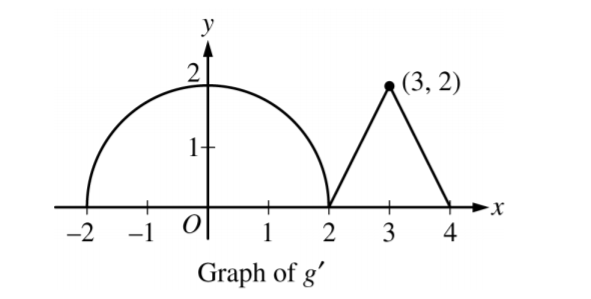
\includegraphics[width=3in]{FEP8.png}
        \end{center}
    The graph of $g'$, the first derivative of the function g, consists of a semicircle of radius $2$ and two line segments, as shown in the figure above. If $g(0) = 1$, what is $g (3)$?
    $$g(3)=g(0)+\int_{0}^{3} g'(x)\, dx = \boxed{\pi + 2}$$
    \item $\int \frac{1+3x}{(1-x)(3x-5)}\,dx = $
    $$\int \frac{1+3x}{(1-x)(3x-5)}\,dx = \int \Bigg( \frac{2}{x-1}-\frac{9}{3x-5}\Biggr) \, dx  = \boxed{2\ln|x-1|-3\ln|3x-5|+C}$$
    \item A spherical snowball is melting in such a way that it maintains its shape. The snowball is decreasing in volume at a constant rate of $8$ cubic centimeters per hour. At what rate, in centimeters per hour, is the radius of the snowball decreasing at the instant when the radius is $10$ centimeters?
    \begin{enumerate}
        \item $\frac{dV}{dt} = -8 \frac{\text{cm}^3}{{\text{hr}^2}}$
        \item $V=\frac{4}{3}\pi r^3$
    \end{enumerate}
    $$\frac{dV}{dt} = 4\pi r^2 \cdot \frac{dr}{dt} \Longrightarrow  \frac{dr}{dt}=\frac{dV}{dt} \cdot \frac{1}{4\pi r^2}$$
    $$\frac{dr}{dt}\bigg\rvert_{r=10} = \boxed{\frac{-1}{50\pi} \frac{\text{cm}}{{\text{hr}}}}$$
    \item If $f(x)=\int_{0}^{x^3} \cos(t^2)\,dt$, then $f'(\sqrt{\pi})=$
    $$f'(x)=\frac{d}{dx}\biggr(F(x^3)-F(0)\biggr) = 3x^2\cos(x^6)$$
    $$\boxed{f'(\sqrt{\pi}) = 3\pi \cos (\pi^3)}$$
    \item Let $g$ be a twice-differentiable, increasing function of t. If $g(0) = 20$ and $g(10) = 220$, which of the following must be true on the interval $0 < t < 10$?
    $$\boxed{g'(t) = 20 \text{ for some $t$ in the interval.}}$$
    \item $\int \frac{6x^2-4x-25}{x-2} \, dx = $
    $$\int \frac{6x^2-4x-25}{x-2} \, dx = \int \biggr(6x+8 -\frac{9}{x-2}\bigg) \, dx = 3x^3+8x -9\ln|x-2|+C$$
    \item The length of the curve  $y = \sin x$ from $x = 0$ to $x = \frac{3\pi}{4}$ is given by
    \begin{enumerate}
        \item $y' = \cos x$
    \end{enumerate}
    $$\boxed{\int_{0}^{\frac{3\pi}{4}} \sqrt{1+\cos^2 x} \, dx}$$
    \item 
    \begin{table}[h!]
        \centering
        \begin{tabular}{|l||l|l|l|l|l|}
        \hline
        $x$    & 10 & 11 & 12 & 13 & 14 \\ \hline
        $f(x)$ & 5  & 2  & 3  & 6  & 5  \\ \hline
        \end{tabular}
        \end{table}
    The table above gives values of the continuous function $f$ at selected values of $x$. If $f$ has exactly two critical points on the open interval $(10, 14)$, which of the following must be true?
    $$\boxed{f'(12) \neq 0}$$
    \item Let $g$ be a function such that $g(y) > 0$  for all $y$. Which of the following could be a slope field for the differential equation $\frac{dy}{dx}=\big(x^2-1\big)g(y)$?
    \begin{center}
        \boxed{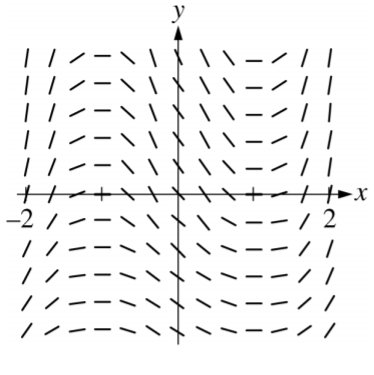
\includegraphics[width=2in]{FEPA6.png}}
    \end{center}
    \item What are all values of $p$ for which $\int_{1}^{\infty}\frac{1}{x^{3p+1}}\,dx$ converges?
    \item The temperature of a solid at time  $t \geq 0$  is modeled by the nonconstant function $H$ and increases according to the differential equation $\frac{dH}{dt}=2H+1$ , where $H(t)$  is measured in degrees Fahrenheit and $t$ is measured in hours. Which of the following must be true?
    $$\int \frac{dH}{2H+1} = \int \, dt \Longrightarrow \frac{1}{2}\ln|2H+1| = t+C \Longrightarrow \boxed{\ln|2H+1| = 2t+C}$$
    \item 
        \begin{center}
            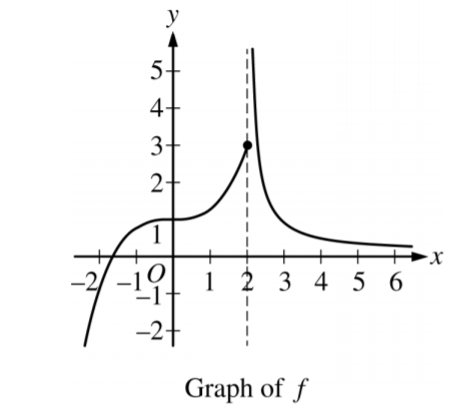
\includegraphics[width=3in]{FEP9.png}
        \end{center}
    The graph of the function $f$ is shown in the figure above. Which of the following statements must be false?
    $$\boxed{\lim_{x\to2} f(x)= f(2)}$$
    \item The rate at which water leaks from a tank, in gallons per hour, is modeled by $R$, a differentiable function of the number of hours after the leak is discovered. Which of the following is the best interpretation of $R'(3)$?\\\\
    \noindent\fbox{\parbox{\textwidth}{The rate of change of the rate at which water leaks from the tank, in gallons per hour per hour, three hours after the leak is discovered.}}
    \item On a certain day, the temperature, in degrees Fahrenheit, in a small town $t$ hours after midnight $(t= 0)$  is modeled by the function $g(t) = 65 - 8\sin \bigg(\frac{\pi t}{12}\bigg)$. What is the average temperature in the town between 3 A.M. $(t= 3)$  and 6 A.M. $(t= 6)$, in degrees Fahrenheit?
    $$\boxed{\frac{1}{3}\int_{3}^{6} g(t)\, dt \approx 57.797 }$$
    \item 
    \begin{table}[h!]
        \centering
        \begin{tabular}{|l||l|l|l|l|l|}
        \hline
        $x$    & 0.0 & 0.5 & 1.0 & 1.5 & 2.0 \\ \hline
        $f(x)$ & 1.0  & 0.7  & 0.5  & 0.4  & 0.3  \\ \hline
        \end{tabular}
        \end{table}
    Let $y = f(x)$  be the solution to the differential equation $\frac{dy}{dx}=f'(x)$ with initial condition  $f(1) = 5$. Selected values of $f'(x)$  are given in the table above. What is the approximation for $f(2)$  if Euler's method is used with a step size of 0.5, starting at $x= 1$?
    \begin{table}[h]
        \centering
        \caption{$\Delta x = 0.5$}
        \begin{tabular}{l|l|l|l}
        $x$ & \multicolumn{1}{l|}{$y$} & \multicolumn{1}{l|}{$\frac{dy}{dx}$} & $\Delta y$ \\ \hline
        1 & 5 & 0.5 & 0.25 \\
        1.5 & 5.25 & 0.4 & 0.2 \\
        2 & 5.45 &  & 
        \end{tabular}
        \end{table}
        $$f(3)\approx 3.75 = \boxed{5.45}$$
    \item The first derivative of the function $f$ is defined by $f'(x) = (x^2 +1)\sin(3x - 1)$ for $-1.5 < x < 1.5$. On which of the following intervals is the graph of $f$ concave up?
    $$\boxed{(-1.5, -1.341) \text{ and } (-0.240, 0.964)}$$
    \item For  $t \geq 0$, the velocity of a particle moving along the $x$-axis is given by  $v(t) =t^3-6t^2+ 10t- 4$. At what time $t$ does the direction of motion of the particle change from right to left?
    $$\boxed{t=2.000}$$
    \item Let $f$ be a function such that $f (1) = -2$ and $f (5) = 7$. Which of the following conditions ensures that $f(c) = 0$ for some value $c$ in the open interval $(1,5)$?
    $$\boxed{\text{$f$ is continuous on the closed interval $[1, 5]$.}}$$
    \item 
        \begin{center}
            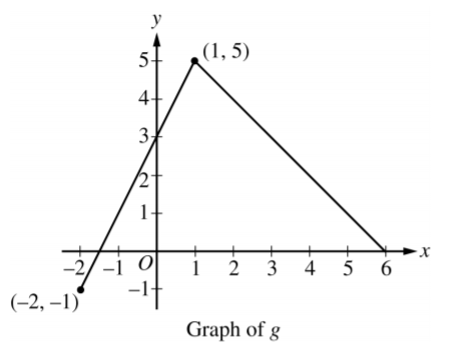
\includegraphics[width=2in]{FEP10.png}
        \end{center}
    The graph of the function $g$ is shown above. If $f$ is the function given by $f(x) =g(g(x))$ , what is the value of  $f'(0)$?
    $$f'(x)=g'(g(x))\cdot g'(x)$$  
    $$f'(0)= g'(3)\cdot g'(0) = 2 \cdot -1 = \boxed{-2}$$
    \item Let $f$ be a function such that $f(-x) = -f(x)$  for all $x$. If $\int_{0}^{2} f(x) \, dx = 5$, then $\int_{-2}^{2}\big(f(x)+6\big) \, dx$
    $$\int_{-2}^{2}\big(f(x)+6\big) \, dx =\int_{-2}^{2} f(x)\, dx + \int_{-2}^{2} 6 \, dx $$
    $$\int_{-2}^{2} f(x)\, dx = 0$$
    $$\Longrightarrow 6x \biggr\rvert_{-2}^{2} =\boxed{24}$$
    \item 
        \begin{center}
            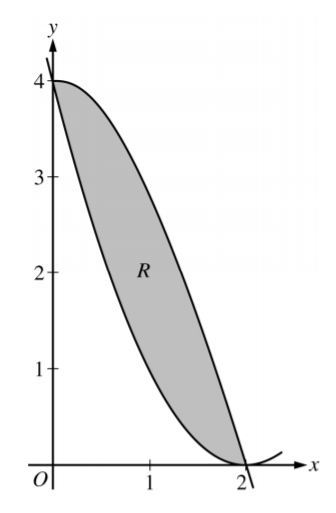
\includegraphics[width=3in]{FEP 11.png}
        \end{center}
     Let $R$ be the region in the first quadrant bounded by the graphs of $y = 4 \cos \bigg(\frac{\pi x}{4}\bigg)$ and $y = (x-2)^2$, as shown in the figure above. The region $R$ is the base of a solid. For the solid, each cross section perpendicular to the $x$-axis is an isosceles right triangle with a leg in region $R$. What is the volume of the solid?
     $$\boxed{V=\frac{1}{2}\int_{0}^{2} \biggr(4 \cos \bigg(\frac{\pi x}{4}\bigg) - (x-2)^2\bigg)^2\, dx = \frac{8(7\pi^3 -160\pi+320)}{5\pi^3}\approx 1.775}$$
\end{enumerate}
\end{document}
